\documentclass[12pt]{article}

\usepackage[utf8]{inputenc}
\usepackage[ngerman]{babel}
\usepackage{csquotes}
\MakeOuterQuote{"}

\usepackage[backend=biber,style=reading]{biblatex}
\addbibresource{../literature.bib}

\usepackage[margin=2cm]{geometry}

\usepackage{wrapfig}
\usepackage{caption}

\usepackage[table]{xcolor}
\usepackage{tabularx}

\usepackage{hyperref}
\hypersetup{colorlinks=true, linkcolor=blue, linktocpage}

\usepackage{minted}
% rubber: shell_escape

\usepackage{fontawesome}

\usepackage[most]{tcolorbox}

\newtcolorbox{defbox}[2][]{colback=yellow!5!white,
colframe=yellow!75!black,fonttitle=\bfseries,
colbacktitle=yellow!85!black,enhanced,
attach boxed title to top left={yshift=-0.03cm},
title={#2},#1}

\newtcolorbox{aufgbox}[2][]{colback=blue!5!white,
colframe=blue!75!black,fonttitle=\bfseries,
colbacktitle=blue!85!black,enhanced,
attach boxed title to top left={yshift=-0.03cm},
title={#2},#1}

\newtcolorbox{expbox}[2][]{colback=orange!5!white,
colframe=orange!75!black, enhanced, #1}

\newtcolorbox{graycode}[2][]{colback=gray!5!white,
colframe=gray!75!black, enhanced, #1}

\usepackage{setspace}
\onehalfspace

% Those are used for showkeys long key splitting, as described in
% https://tex.stackexchange.com/a/311421/1280, but may be otherwise
% come in handy.
\usepackage{seqsplit}
\usepackage{xstring}

\usepackage{graphicx}
\usepackage{standalone}
\usepackage{pdfcomment}

\usepackage{tikz}
\usetikzlibrary{
  arrows.meta,
  calc,
  positioning,
  decorations.pathreplacing,
  tikzmark,
}

\newcommand\kariert[2][0.5cm]{%
  \begin{tikzpicture}[gray, step=#1]
    \pgfmathtruncatemacro\anzahl{(\linewidth-\pgflinewidth)/#1} % maximale Anzahl Kästchen pro Zeile
    \draw (0, 0) rectangle (\anzahl*#1, #2*#1) (0, 0) grid (\anzahl*#1, #2*#1);
  \end{tikzpicture}
}

\usepackage[school]{pgf-umlcd}

% rubber: watch arbeitsheft.acn
% rubber: watch arbeitsheft.acr
\usepackage[acronym]{glossaries}
\makeglossaries

\newacronym{SOS}{SOS}{School Operating System}
\newacronym{UID}{UID}{Benutzerkennung}
\newacronym{GID}{GID}{Gruppenkennung}
\newacronym{PID}{PID}{Prozessnummer}
\newacronym{ZSL}{ZSL}{Zugriffssteuerungsliste}
\newacronym{CWD}{CWD}{Curent Working Directory}

% \bibliography{bibliography}

\makeatletter
\@ifundefined{MyEnableAnnotations}
  {%
    \def\MyEnableAnnotations{false}
  }
  {%
  }
\makeatother
\newtoggle{disableAnnotations}
\ifthenelse{\equal{\MyEnableAnnotations}{false}}{
  \toggletrue{disableAnnotations}
}{}
\nottoggle{disableAnnotations}{
  \NewDocumentCommand \annotate {m m m}{\pdfmarkupcomment[author=#3]{#1}{#2}}
  \NewDocumentCommand \remark {m m}{\pdfcomment[author=#2]{#1}}
  \NewDocumentCommand \inlineremark {m m o}{\pdfmarkupcomment[author=#1,color=yellow]{[#2]}{#3}}
  \NewDocumentCommand \inlinetodo {m}{\pdfmarkupcomment[color=yellow]{[TODO: #1]}}

  % Use showkeys if annotations are enabled.
  % Source https://tex.stackexchange.com/a/311421/1280
  % with minor modifcations, i.e. 1.2 times \marginparwidth
  % \usepackage{showkeys}
  % \renewcommand*\showkeyslabelformat[1]{%
  %   \noexpandarg%
  %   % instead of \textvisiblespace you can also put in ~
  %   % if you want to keep a plain space at space characters
  %   \StrSubstitute{\(\{\)#1\(\}\)}{ }{\textvisiblespace}[\TEMP]%
  %   \parbox[t]{1.2\marginparwidth}{\raggedright\normalfont\small\ttfamily\expandafter\seqsplit\expandafter{\TEMP}}}
}{
  \NewDocumentCommand \annotate {m m m}{}
  \NewDocumentCommand \remark {m m}{}
  \NewDocumentCommand \inlineremark {m m o}{}
  \NewDocumentCommand \inlinetodo {m}{}
}

\NewDocumentCommand \ifAnnotationsEnabled {m}{\nottoggle{disableAnnotations}{#1}{}}

\usepackage{titling}
\usepackage{fancyhdr}

\usepackage[german]{cleveref}

\author{Florian Fischer}
\title{Arbeitsheft Betriebsysteme}

\definecolor{inlinecodeboxbackgroundcolor}{HTML}{F8F8F8}
\definecolor{inlinecodeboxframecolor}{HTML}{DDDDDD}

% inlinecode command for including code snippets inline
% (fake verbatim, so all special character should be escaped,
% or textmode equivalents of special characters should be used)
\newcommand{\inlinecode}[1]{%
  \begin{tikzpicture}[baseline=0ex]%
    \node[anchor=base,%
      text height=1em,%
      text depth=1ex,%
      inner ysep=0pt,%
      draw=inlinecodeboxframecolor,%
      fill=inlinecodeboxbackgroundcolor,%
      rounded corners=2pt] at (0,0) {\footnotesize\texttt{#1}};%
  \end{tikzpicture}%
}

\newcommand{\boldred}[1]{\textbf{\textcolor{red}{#1}}}

\fancyhf{}
\fancyhf[HC]{\thetitle}
\fancyhf[HL]{SOS}
\fancyhf[FC]{\thepage}

\begin{document}
\pagestyle{empty}
% \maketitle
\begin{titlepage}
\setlength\parindent{0pt}
\vspace{3cm}
{\huge \textbf{SOS - Hilfe was ist hier los?}}
\vspace{1.5cm}

{\Large \textbf{Anleitung zum School Operating System.}}
\vspace{1cm}
\hrule
\vspace{1cm}
\begin{centering}
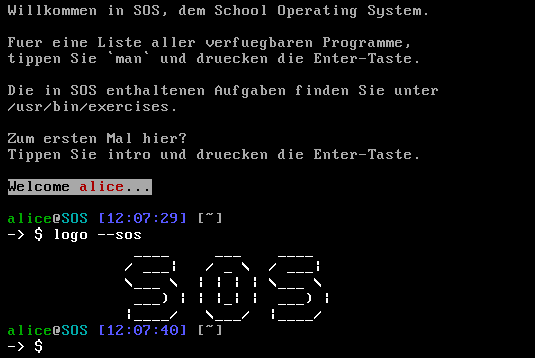
\includegraphics[keepaspectratio, width=\textwidth]{logo.png}
\end{centering}
\hrule
\vspace{1cm}
{\large \textbf{Arbeitsheft zum Thema Betriebsysteme}}

\end{titlepage}

\newpage
\pagestyle{fancy}
\pagenumbering{roman}

\tableofcontents
\vfill{}
{
\onehalfspacing
\setlength\parindent{0pt}
\textbf{\large Konzeption des Arbeitshefts}: \\[0.3cm]

Das Arbeitsheft begleitet den Einsatz des \gls{SOS} im Unterricht, das die Grundlagen und Aufgaben von Betriebssystemen nach dem Lehrplan der 12. Jahrgangsstufe mit erhöhtem Anforderungsbereich behandelt. \\[0.2cm]

\textbf{\theauthor} \\
Hans-Sachs-Gymnasium Nürnberg \\
E-Mail: \href{mailto:florian.fischer@muhq.space}{florian.fischer@muhq.space} \\[0.2cm]

Dieses Arbeitsheft ist lizenziert unter einer \href{https://creativecommons.org/licenses/by-sa/4.0/}{Creative Commons CC BY-SA Lizenz} (Namensnennung – Weitergabe unter gleichen Bedingungen).
}


\newpage
\pagenumbering{arabic}

\section*{Über \gls{SOS} und dieses Arbeitsheft}

Dieses Arbeitsheft kann als Begleitung oder als Inspiration in Kombination mit \gls{SOS} im Unterricht eingesetzt werden.

\subsection*{\acrfull{SOS}}

Bei \gls{SOS}, handelt es sich um eine Kombination aus einer portable virtuellen Maschine (\href{https://www.qemu.org/}{QEMU}) und dem von der Universität Verona entwickelten und für \gls{SOS} und den Informatikunterricht angepassten Betriebssystem \href{https://mentos-team.github.io/}{MentOS}.

\subsubsection*{Ziele}

Betriebssysteme sind in unserem digitalen Alltag allgegenwärtig.
Dennoch ist dieser Fakt den meisten Anwenderinnen nicht bewusst, was dafür spricht, dass moderne Betriebssysteme ihrer Aufgabe nachkommen die einfache und sichere Benutzung der unterschiedlichsten Geräte von Smartwatches, über Mobiltelefone zu klassischen PCs reibungslos zu ermöglichen.

\gls{SOS} dient dazu die oft schwer erfahrbaren Aufgaben von Betriebssystemen erlebbar zu machen.
Es werden die wichtigsten und universellen Begriffe im Kontext von Betriebssystemen wiederholt und veranschaulicht.
Besonderer Fokus liegt dabei auf der Gewährleistung eines sicheren Betrieb, durch die Verwaltung und Durchsetzung von Berechtigungen, im Dateisystem.

Außerdem, lädt \href{https://github.com/mentos-team/MentOS}{MentOS} durch seine verhältnismäßigen einfachen Aufbau, sowie die vorhandene \href{https://mentos-team.github.io/doc/doxygen/index.html}{Dokumentation} dazu ein Neues zu entdecken und weiterführendes Interesse zu wecken und in gewissen Umfang auch zu befriedigen.

\subsubsection*{Benutzung}

\gls{SOS} ist so konzipiert, dass die Benutzung im Unterricht möglichst einfach ist.

\begin{enumerate}
\item Eine einsatzfähige Version von \gls{SOS} inklusive aller Arbeitsmaterialien kann unter \\ \href{github.com/fischerling/releases}{https://github.com/fischerling/SOS/releases} direkt herunterzuladen werden.
Die Datei \\ \inlinecode{sos-win.zip} enthält alle benötigten Komponenten zum Einsatz von \gls{SOS}.
\item Zur Benutzung von \gls{SOS} muss das heruntergeladene Archiv komplett extrahiert werden.
\item Um das Betriebssystem in der enthaltenen virtuellen Maschine zu starten, reicht es die Datei \inlinecode{run.bat} durch Doppelklick auszuführen.
Gegebenenfalls muss eines Sicherheitswarnung von Windows, bestätigt werden.
\item Nachdem MentOS in der virtuellen Maschine gestartet ist, wird der Nutzer nach einem Login, wie in \Cref{fig:login} dargestellt, gefragt.
\begin{figure}
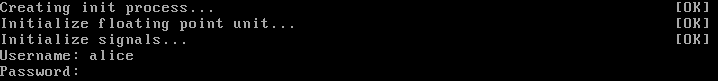
\includegraphics[keepaspectratio, width=\textwidth]{login_prompt.png}
\caption{Login-Aufforderung von MentOS}
\label{fig:login}
\end{figure}
Alle Aufgaben in \gls{SOS} sind für den Benutzer \inlinecode{alice} mit Passwort \inlinecode{alice} ausgelegt.
\item \label{sec:start_exercise} Übungsaufgaben in \gls{SOS} bestehen meist aus zwei Programmen.
Ein \inlinecode{setup} Programm bereitet den Zustand des Systems für die Aufgabe vor.
Das \inlinecode{checkup} Programm dient dazu den Bearbeitungsstand der Aufgabe interaktiv zu überprüfen.
Die Aufgaben Programme sind im Dateisystem unter \inlinecode{/usr/bin/exercises/} zu finden.
\end{enumerate}

\newpage
\section{Grundlagen und erste Schritte}

\begin{defbox}{Betriebssystem}
Das Betriebssystem ist im vereinfachtem Sinn die Software die im privilegierten \textit{kernel modus}, der Hardware ausgeführt wird, siehe \Cref{fig:stack}.
Dies muss aber nicht immer der Fall sein.
Grundsätzlich hat das Betriebssystem, die Aufgabe die bestehende Hardware den Nutzerprogrammen in geeigneter Weise zur Verfügung zustellen und deren sichere Verwendung zu gewährleisten.
\end{defbox}

\begin{wrapfigure}{r}{8.5cm}
\begin{tikzpicture}[layer/.style={draw, minimum width=5cm, minimum height=1cm}]
\node[layer, fill=gray] (h) {};
\node[layer, above=0cm of h] (os) {Betriebssystem};
\node[layer, above=0cm of os] (shell) {Nutzerschnittstelle};
\node[layer, above=0cm of shell] (utils) {};

\node[draw, circle, fill=gray!70, minimum size=0.5cm, above=0.25cm of shell, xshift=-1.2cm] (u1) {};
\node[draw, circle, fill=gray!70, minimum size=0.5cm, above=0.25cm of shell] (u2) {};
\node[draw, circle, fill=gray!70, minimum size=0.5cm, above=0.25cm of shell, xshift=1.2cm] (u3) {};

\draw[Latex-] (u1) -- ($(u1) + (-1.8, 1)$) node[above, text width=1cm] {\small Webbrowser}; 
\draw[Latex-] (u2) -- ($(u2) + (0, 1)$) node[above, align=center, text width=2cm] {\small E-Mail Programm};
\draw[Latex-] (u3) -- ($(u3) + (0.75, 1)$) node[above, text width=1cm] {\small Mediaplayer}; 

\draw[decoration={brace, raise=3pt}, decorate]
  (h.north east) -- node[right, xshift=0.2cm] {Hardware} (h.south east);
\draw[decoration={brace, raise=3pt}, decorate]
  (utils.north east) -- node[right, xshift=0.2cm] {Software} (h.north east);
\draw[decoration={brace, mirror, raise=3pt}, decorate]
  (os.north west) -- node[left, xshift=-0.2cm] {kernel mode} (os.south west);
\draw[decoration={brace, raise=3pt}, decorate]
  (shell.south west) -- node[left, xshift=-0.2cm] {user mode} (utils.north west);
\end{tikzpicture}

\caption{Platz des Betriebssystem im Stapel der Technologien.}
\label{fig:stack}
\end{wrapfigure}

Die Hauptaufgabe des Betriebssystem ist demnach die Verwaltung und Bereitstellung der vorhandenen Hardwareressourcen, wie der Rechenzeit auf den Rechenkernen, den Hauptspeicher, sowie Zugriff auf Peripherie-Geräte wie das Netzwerk, Festplatten oder Ein-/ und Ausgabegeräte.

\label{sec:security_safety}
Dabei muss das Betriebssystem, die Sicherheit der Ressourcen (englisch \emph{security}) gegen bösartige Dritte, andere Nutzer auf dem System, Schadsoftware, Angriffe über die angeschlossenen Peripherie-Geräte, zumeist das Netzwerk, sicherstellen.

Darüber hinaus ist es auch Aufgabe des Betriebssystems die Betriebssicherheit (englisch \emph{safety}) zu gewährleisteten, dass heißt beispielsweise den Verlust von Daten, oder das Abstürzen des Systems bei einem Fehler zu verhindern.

Um diese Schutzziele zu erfüllen arbeitet das Betriebssystem eng mit der verfügbaren Hardware zusammen.
Diese erlaubt es beispielsweise durch die Trennung des Ausführung in \textit{user mode} und \textit{kernel mode}, gewisse Operationen auf das Betriebssystem einzuschränken.
Darüber hinaus sorgt die Hardware nach Instruktion durch das Betriebssystem dafür, dass Programme nur auf ihren eigenen exklusiven Speicherbereich und nicht den anderer Programme zugreifen können.
Das schützt sowohl das gesamte System vor Fehler in einzelnen Programmen, sowie das einzelne Programm vor dem böswilligen Zugriff Dritter.

\begin{aufgbox}{Arbeitsauftrag: Los gehts!}
\begin{wrapfigure}[11]{r}{8.5cm}
\centering
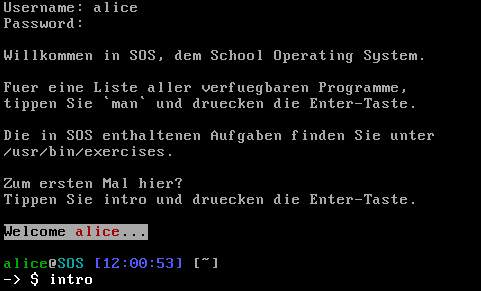
\includegraphics[keepaspectratio, width=8cm]{intro_prompt.png}
\caption{Starten des \texttt{intro} Programms, nach erfolgreicher Anmeldung.}
\label{fig:intro_start}
\end{wrapfigure}

Um den Umgang mit dem rein textbasierten \gls{SOS} zu üben und einige grundlegende Konzepte aus der Welt der Betriebssysteme zu erkunden, stellt \gls{SOS} ein \inlinecode{intro} Programm zur Verfügung.
\begin{enumerate}
\item Starten Sie, falls noch nicht geschehen, \gls{SOS} durch Ausführen der Datei \inlinecode{run.bat}.
\item Melden Sie sich als der Benutzer \inlinecode{alice} mit dem Passwort \inlinecode{Alice} an.
\item Starten Sie nach einer erfolgreichen Anmeldung, wie in \Cref{fig:intro_start} gezeigt, das \inlinecode{intro} Programm durch Eintippen des Namens und Drücken der Enter-Taste. 
\end{enumerate}
\end{aufgbox}

Im Folgenden werden die Konzepte in der Reihenfolge in der sie im Ablauf des \texttt{intro}-Programms auftauchen beschrieben.

\subsection{Prozesse}

Eines der fundamentalsten Konzepte eines Betriebssystem ist der Prozess.
Ein Prozess repräsentiert ein laufendes Programm.
Diese Abstraktion erlaubt es mehrere Programme scheinbar gleichzeitig auf nur einem Rechenkern auszuführen.

\begin{defbox}[breakable]{Prozess}
\begin{wrapfigure}[11]{r}{4.5cm}
\vspace{-0.5cm}
\begin{tikzpicture}
\begin{class}[text width=4cm]{PROZESS}{0,4}
\attribute{Zustand}
\attribute{Besitzer}
\attribute{Argumente}
\attribute{CWD}
\attribute{Elternprozess}
\attribute{Ausgabe-Streams}
\end{class}
\end{tikzpicture}
\caption{Vereinfachte Klassenkarte eines Prozesses}
\label{fig:proccess_class}
\end{wrapfigure}

Ein Prozess besteht aus allen Datenstrukturen, die benötigt werden um ein Programm auszuführen, beispielsweise einem exklusiven Speicherbereich, sowie dem auszuführenden Programmcode.
Jeder Prozess hat einen \emph{Zustand}, anhand dessen der Prozess in der Ablaufplanung des Betriebssystem, berücksichtigt wird.
Wartet ein Prozess auf Daten von der Festplatte wird er von der Ablaufplanung ausgenommen bis die Daten vorhanden sind.

Um die Sicherheit des Systems zu gewährleisten hat jeder Prozess zugewiesene Berechtigungen, herkömmlich und so auch in \gls{SOS} sind die Berechtigungen mit dem \emph{Besitzer} und der Gruppe des Prozesses verbunden.
Die \gls{UID} und \gls{GID} eines Prozesses werden beim Erstellen des Prozesses vom \emph{Elternprozess} geerbt.
Da ein Prozess immer nur von einem anderen Prozess erzeugt werden kann, bilden alle Prozesse des Systems einen Baum.
Wobei die Wurzel des Baums, der \texttt{init}-Prozess mit \gls{PID} 1 vom Betriebssystem gestartet wird.
\end{defbox}

Die \emph{Kommandozeile} ermöglicht die rein textbasierte Benutzung des Computer, das heißt die Erzeugung und Kontrolle von Prozessen.
Ein \inlinecode{shell} genanntes Programm, liest Zeile für Zeile Befehle des Nutzers ein.
Jede Zeile wird dabei anhand der enthaltenen Leerzeichen getrennt.

\begin{wrapfigure}[7]{l}{6cm}
\vspace{-0.75cm}
\begin{expbox}{}
Programme werden anhand ihres Namens in Verzeichnissen, im \texttt{Suchpfad}\\
(UNIX: \texttt{\$PATH}; Windows: \texttt{Path}) gesucht.
\end{expbox}
\end{wrapfigure}

Das erste Wort der Zeile wird als Name eines Programms interpretiert.
Es wird ein neuer Prozess gestartet, dieser führt das Programm das anhand des Namens gefunden wurde aus.
Der Rest der Zeile wird dem neuen Programm als \emph{Argumente} übergeben.

Jeder Prozess hat ein Verzeichnis zugewiesen in dem er aktuell "arbeitet" und von dem aus alle \hyperref[sec:rel_paths]{relativen Dateipfade} interpretiert werden.
Dieses "Arbeitsverzeichnis" wird englisch \gls{CWD} genannt.
Das \gls{CWD} wird von dem Prozess der den neuen Prozess startet, dem \emph{Elternprozess} geerbt.
In der shell kann das \gls{CWD} mit dem Befehl \inlinecode{cd} (englisch \textcolor{red}{c}hange \textcolor{red}{d}irectory) geändert werden.

% Mehrbenutzerbetrieb

\subsection{Dateien}

Ein weiteres essentielles Konzept nahezu aller Betriebssysteme ist die \emph{Datei}.
Um die Eigenheiten verschiedener persistenter Speichermedien, von Festplatten, über USB-Sticks bis hin zu Magnetbändern, zu verstecken, bieten Betriebssysteme das Konzept von Dateien an.
Um Dateien zu strukturieren werden besondere Dateien sogenannte Verzeichnisse (englisch \emph{directory}) verwendet.
Ähnlich zu Prozessen können Dateien in einem Dateisystem in einer Baumstruktur gruppiert werden (vergleiche \Cref{fig:fs_tree}).

\begin{defbox}[breakable]{Datei}
\begin{wrapfigure}[8]{r}{4.5cm}
\vspace{-0.5cm}
\begin{tikzpicture}
\begin{class}[text width=4cm]{DATEI}{0,4}
\attribute{Name}
\attribute{Typ}
\attribute{Größe}
\attribute{Besitzer}
\attribute{Berechtigungen}
\end{class}
\end{tikzpicture}
\caption{Vereinfachte Klassenkarte einer Datei}
\label{fig:file_class}
\end{wrapfigure}
Die gängigste Umsetzung von Dateien ist sie als Folge von Bytes bekannter \emph{Größe} zu behandeln.
Der Inhalt einer Datei hat für das Betriebssystem normalerweise keine Bedeutung und muss von Nutzerprogrammen selbst interpretiert werden.
Dateien unterscheiden sich zum Speicherbereich eines Prozesses dadurch, dass sie nach der Beendigung des Prozesses weiter existieren und von mehreren Prozessen und sogar nach einem Neustart des Systems verwendet werden kann.
Um Dateien unterscheiden und wiederverwenden zu können ist jeder Datei ein \emph{Name} zu geordnet.
Manche Betriebssysteme schränken die erlaubten Zeichen in Dateinamen ein.
\end{defbox}

% In einem Betriebssystem existieren unterschiedliche Arten von Dateien, wie das Attribut \emph{Typ} in der Klassenkarte in \Cref{fig:file_class} vermuten lässt:
% \begin{itemize}
% \item reguläre Dateien, die eine Folge von Byte speichern
% \item Verzeichnisse, die die Name anderer Dateien, die in diesem Verzeichnis enthalten sind, speichern
% \item sowie andere \emph{spezielle} Dateien, die beispielsweise die Hardware oder die Ausgaben eines Prozesses als Folge von Bytes zur Verfügung stellen
% \end{itemize}

Da in einem System mehrere Dateien mit dem gleichen Namen existieren können, wird um eine bestimmte Datei verwenden zu können nicht nur ihr Name sondern auch ihr Ort im Dateisystem benötigt.

\begin{wrapfigure}[8]{l}{5.5cm}
\vspace{-0.5cm}
\begin{expbox}
\emph{absolut}: \\
\phantom{ }\hspace{0.2cm}\texttt{/home/alice/README} \\
\emph{relativ}: \\
\phantom{ }\hspace{0.2cm}\texttt{README} \\
\phantom{ }\hspace{0.2cm}\texttt{../bob} \\
\end{expbox}
\end{wrapfigure}

Der Ort einer Datei kann auf zwei Arten angeben werden als \textbf{absoluter} Pfad oder \textbf{relativer} Pfad.
Ein Pfad besteht aus einer beliebigen Liste an Verzeichnissen und einem optionalen abschließenden Dateinamen, getrennt von \emph{Pfadseparatoren}.
Der Pfadseparator in \gls{SOS} ist wie in allen UNIX-Systemen das Zeichen \inlinecode{\texttt{/}} (in Windows ist der Pfadseparator \inlinecode{\texttt{\textbackslash}}).

\textbf{Absolute} Pfade beginnen immer mit dem Wurzelverzeichnis des Dateisystems (\inlinecode{\texttt{/}} in \gls{SOS}).

\label{sec:rel_path}\textbf{Relative} Pfade werden ausgehend vom aktuellen Arbeitsverzeichnis \gls{CWD} des Prozesses interpretiert.

Jedes Verzeichnis enthält die beiden besonderen Einträge \inlinecode{.} und \inlinecode{..} die zusätzlich zu Namen in Pfaden vorkommen können.
Der besondere Eintrag \inlinecode{.} steht dabei für das Verzeichnis selbst und \inlinecode{..} für das Oberverzeichnis.

\begin{figure}[h]
\centering
\begin{tikzpicture}[
  dir/.style={align=left, draw, minimum size = 2cm},
  file/.style={align=left, draw, rounded corners=10pt, minimum size=2cm}
]
\node[dir] (r) {/ \\ root:root \\ \texttt{\textcolor{red}{d}rwxr-xr-x}};
\node[right=of r, dir] (d) {$verzeichnis_1$ \\ owner:group \\ \texttt{\textcolor{red}{d}rwxr-xr-x}};
\draw (r) -- (d);
\node[right=of d, file] (f) {$datei_1$ \\ owner:group \\ \texttt{rw-r-{}-r-{}-}};
\draw (f) -- (d);
\end{tikzpicture}
\caption{Darstellung der Baumstruktur eines Dateisystems ausgehend vom Wurzelverzeichnis~\protect\inlinecode{/}. Ob es sich bei einer Datei um ein  Verzeichnis handelt, wird in der Darstellung der Berechtigungen mit einem vorangestellten \textcolor{red}{d} symbolisiert. Der absolute Pfad von $datei_1$ lautet \protect\inlinecode{/$verzeichnis_1$/$datei_1$}.}
\label{fig:fs_tree}
\end{figure}

\section{Datei-Berechtigungen}

Um die beiden \hyperref[sec:security_safety]{Sicherheits-Schutzziele} \emph{security} und \emph{safety} zu gewährleisten haben Dateien einen \emph{Besitzer} und eine feste Zuweisung an \emph{Berechtigungen}.
Diese Berechtigungen werden bei der Verwendung einer Datei überprüft und die Operation gegebenenfalls vom Betriebssystem abgelehnt.

\begin{defbox}{Datei-Berechtigungen}
\begin{wrapfigure}{r}{8cm}
\begin{tikzpicture}

\node (u) {\texttt{rwx}};
\node[right=0pt of u] (g) {\texttt{rw-}};
\node[right=0pt of g] (o) {\texttt{r-{}-}};

\coordinate (repr) at (-0.8, 0);
\node[anchor=east] at (repr |- u){symbolisch};

\coordinate (brackets) at (0, 0.2);
\coordinate (lbrackets) at (0, -0.2);
\node[above = 1.5cm of u] (ul) {Owner};
\draw (u.west) -- (u.west |- brackets) -- (u.east |- brackets) -- (u.east);
\node[above = 1cm of g] (gl) {Group};
\draw (g.west) -- (g.west |- brackets) -- (g.east |- brackets) -- (g.east);
\node[above = 0.5cm of o] (ol) {Other};
\draw (o.west) -- (o.west |- brackets) -- (o.east |- brackets) -- (o.east);

\node[right = 1.5cm of g] (expl) {\texttt{rwx}};
\draw[dashed] (expl.west) -- (expl.west |- lbrackets) -- (expl.east |- lbrackets) -- (expl.east);
\draw[dashed] (expl.south) -- ($(expl.south) - (0, 0.15)$) -- ($(o.south) - (0, 0.15)$) -- (o.south);
\draw[dashed] (o.west) -- (o.west |- lbrackets) -- (o.east |- lbrackets) -- (o.east);

\node[anchor=west] (rexpl) at (expl.east |- ul) {\textbf{r}ead};
\draw ($(expl.north) - (0.2, 0)$) |- (rexpl);
\node[anchor=west] (wexpl) at (expl.east |- gl) {\textbf{w}rite};
\draw (expl) |- (wexpl);
\node[anchor=west] (xexpl) at (expl.east |- ol) {e\textbf{x}ecute};
\draw ($(expl.north) + (0.2, 0)$) |- (xexpl);

\node[above = of gl] {Berechtigungsklassen};

\node[below =  0.2cm of u] (ub) {\texttt{111}};
\node[below =  0.2cm of g] (gb) {\texttt{110}};
\node[below =  0.2cm of o] (ob) {\texttt{100}};
\node[anchor=east] at (repr |- ub){binär};

\node[below =  0.2cm of ub] (uo) {\texttt{07}};
\node[below =  0.2cm of gb] (go) {\texttt{06}};
\node[below =  0.2cm of ob] (oo) {\texttt{04}};
\node[anchor=east] at (repr |- uo){oktal};

\draw (u) -- (ul);
\draw (g) -- (gl);
\draw (o) -- (ol);
\end{tikzpicture}

\caption{Berechtigungs-Bits einer Datei gegliedert nach den Berechtigungsklassen}
\label{fig:filePermissions}
\end{wrapfigure}

Eine sehr rudimentäre, aber dennoch in UNIX-ähnlichen System, wie Linux, weit verbreitete, Art die Berechtigungen einer Datei zu verwalten, ist diese in \underline{neun Bit} zu speichern.
Diese Bits werden, wie \Cref{fig:filePermissions} dargestellt, in drei Klassen a drei Bits aufgeteilt.
Die Klassen stehen für den Besitzer der Datei, die Gruppenkennung der Datei, sowie alle anderen.

Das erste Bit (\boldred{r}ead) innerhalb einer Klasse gibt an, ob die Datei gelesen werden darf.
Das zweite Bit (\boldred{w}rite) regelt, ob die Datei geschrieben werden darf.
Das dritte Bit (e\boldred{x}ute) steuert, ob die Datei in einem Prozess ausgeführt werden darf, oder falls es sich um ein Verzeichnis handelt, ob auf andere Dateien innerhalb des Verzeichnisses zugegriffen werden darf.

Vor der Verwendung einer Datei wird zunächst, die Klasse des Prozesses, der die Datei verwenden möchte bestimmt und anhand derer geprüft, ob die Operation erlaubt ist.
\end{defbox}

Neben den neun grundlegenden Bits für die drei Klassen existieren noch drei zusätzliche Bits für erweiterte Dateiberechtigungen.
Bei dem ersten Bit handelt es sich um das sogenannte "\emph{sticky bit}", das bei von Allen schreibbaren Verzeichnissen, das Löschen verhindert.
Die zwei verbleibenden Bits werden "\emph{SUID}" (\textcolor{red}{S}et \textcolor{red}{UID}) bzw. "\emph{SGID}" (\textcolor{red}{S}et \textcolor{red}{GID}) genannt.
Ist eines dieser Bits gesetzt wird ein Programm mit dem Besitzer bzw. der Gruppe der Programm-Datei statt des Elternprozesses ausgeführt.
Dies wird verwendet um beispielsweise Nutzern kontrollierten Zugriff auf den \emph{root}-Nutzer mit UID 0 zu gewähren.

Das in \gls{SOS} enthaltene Programm \inlinecode{doas} prüft anhand einer Konfigurationsdatei, ob der aktuelle Benutzer die Berechtigung hat Befehle als \emph{root}-Nutzer auszuführen, und führt gegebenenfalls den als Argumente übergebenen Befehl mit \gls{UID} 0 aus.

Modernen Dateisysteme unterstützen darüber hinaus, eine feingranularer Steuerung der Berechtigungen auf Basis einer \gls{ZSL}.

\begin{aufgbox}{Arbeitsauftrag: Berechtigungsbits}
Gängige Berechtigungen für Verzeichnisse sind die Bits \texttt{0755}.
Wandeln Sie die Bits aus der Oktalschreibweise in ihre symbolische Darstellung um und interpretieren Sie ihre Bedeutung. \\[-0.2cm]

\kariert{6}

Untersuchen sie die Berechtigungen der folgenden Dateien:

\begin{tabular}{p{0.233\textwidth} p{0.7\textwidth}}
\begin{enumerate}
  \item \texttt{/bin/doas}
  \item \texttt{/bin/ls}
  \item \texttt{/etc/passwd}
  \item \texttt{/etc/shadow}
  \item \texttt{/home/bob}
\end{enumerate}
&
\vspace{0.01cm}
\kariert{14}
\end{tabular}
\end{aufgbox}

\clearpage
\subsection{Kartographie der Beispiellandschaft}
\gls{SOS} enthält eine Verzeichnisstruktur, in der die Bedeutung der Berechtigungen von Dateien und Verzeichnissen an Beispielen aus der analogen Welt verdeutlicht werden.
Diese wird beim \hyperref[sec:start_exercise]{Start} der \texttt{file-permission}-Aufgaben durch ausführen des Programms \inlinecode{/usr/bin/exercises/file-permissions/setup} angelegt.

\begin{aufgbox}{Arbeitsauftrag: Kartographie der Beispiellandschaft}
Erkunden Sie die Verzeichnisstruktur unter \inlinecode{/home/alice/Landschaft}. 
Zeichnen Sie die Beispiellandschaft als Baumdiagramm (vgl. \Cref{fig:fs_tree}).
Stellen Sie Vermutungen darüber an warum zu einem Beispiel die bestehenden Berechtigungen passen.
Hilfreiche Programme: \inlinecode{ls}, \inlinecode{stat}, \inlinecode{cd}.
\vspace{0.2cm}
\kariert{32}
\end{aufgbox}

\subsection{Kartographie des Dateisystems}
Die Verzeichnisstruktur von \gls{SOS}, die sich am \href{https://refspecs.linuxfoundation.org/FHS_3.0/fhs-3.0.html}{File Hierarchy Standard} für UNIX-ähnlichen Systems orientiert, enthält ganz bestimmte Berechtigungen für gewissen Teilbäume und Dateien.

\begin{aufgbox}{Arbeitsauftrag: Kartographie des Dateisystems}
Erstellen Sie ein Baumdiagramm des Dateisystems von \gls{SOS}.
Färben Sie die Teilbäume entsprechend ihres Besitzers ein und achte Sie dabei auch auf Ausreißer die von den anderen Berechtigungen abweichen und stellen Sie Vermutung an warum dies jeweils der Fall ist.
\vspace{0.2cm}
\kariert{36}
\end{aufgbox}

\subsection{Herausforderung: Geheimnisse}

Oft sind nicht akkurat gepflegte Berechtigungen Ursache für Sicherheitsprobleme.
Erlauben sie es zum Beispiel unbefugten sensible Informationen zu lesen oder in schlimmsten Fall beliebigen Code auszuführen.
\gls{SOS} enthält eine kleine Herausforderung, bei der die Geheimnisse des Nutzers \inlinecode{alice} geschützt und die Geheimnisse des Nutzers \inlinecode{bob} herausbekommen werden müssen.

\begin{aufgbox}{Arbeitsauftrag: Geheimnisse}
Nachdem Start der \texttt{file-permission}-Aufgabe durch Ausführen des Programms \inlinecode{/usr/bin/exercises/file-permissions/setup} enthält das Verzeichnis \inlinecode{/home/alice} die Datei \inlinecode{secrets.txt}, die es zu schützen gilt.
Das Verzeichnis \inlinecode{/home/bob} enthält die Dateien \inlinecode{secrets.txt} und \inlinecode{top\_secret.txt} der Inhalt nötig ist um die Fragen des Programms \inlinecode{/usr/bin/exercises/file-permissions/checkup} erfolgreich zu beantworten.
Reflektieren Sie, die Art und Weise wie sie an die Informationen gelangt sind und ob diese verhindert werden können.
\vspace{0.2cm}

Happy Hacking :)
\vspace{0.2cm}

Dem Autor sind drei Möglichkeiten bekannt, den Inhalt der Datei \inlinecode{top\_secret.txt} zu erfahren.
Der ersten Person die alle drei, oder potenziell noch weitere Möglichkeiten findet und diese unter \href{mailto://sos@muhq.space}{sos@muhq.space} erklärt, verspricht der Autor hiermit ein heiß Getränk ihrer Wahl.
\end{aufgbox}

\printnoidxglossary[type=acronym]
\printacronyms
\end{document}
